\documentclass[../manuale-sviluppatore.tex]{subfiles}

\begin{document}

\subsection{Programma di addestramento}
\label{sub:programma_di_addestramento}

\subsubsection{Aggiunta di nuovi algoritmi di predizione}
\label{ssub:nuovi_algoritmi_di_predizione}
All'interno del programma di addestramento, per gestire i diversi algoritmi di predizione dei dati, è stato utilizzato il design pattern Object Adapter come riportato nella seguente figura.

\begin{figure}[H]
  \centering
  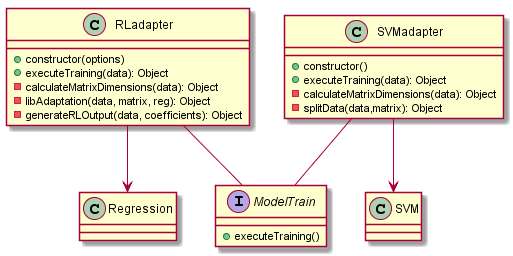
\includegraphics[width=10cm]{img/objectAdapter.png}
  \label{fig:scice_documenti}
  \caption{Object Adapter per gestione degli algoritmi}
\end{figure}

Dalla figura si possono notare le due librerie esterne per la Regressione lineare (Regression) e le Support vector machine (SVM) che vengono adattate creando una propria classe adapter che estende l'interfaccia modelTrain.
Tali classi adapter contengono il metodo executeTraining(data) che deve essere presente in ogni classe adapter essendo il vero metodo che attiva la predizione dei dati raccolti utilizzando lo specifico algoritmo che adatta, può poi contenere altre funzioni
private utili per essere utilizzate all'interno del metodo executeTraining(data) per facilitare l'addestramento dei dati, senza quindi andare a modificare la libreria dell'algoritmo scelto.
\\ \\
Nel caso quindi si volesse includere un nuovo algoritmo di predizione dei dati i passaggi da svolgere per attuare tale cambiamento sono:
\begin{enumerate}
  \item Inserire la libreria esterna relativa all'algoritmo di predizione che si desidera implementare, all'interno del package vendor dell'applicazione;
            \begin{figure}[H]
              \centering
              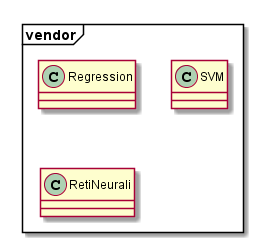
\includegraphics[width=6cm]{img/packagesRetiNeurali.png}
              \label{fig:scice_documenti}
              \caption{Esempio con la libreria sulle Reti neurali}
            \end{figure}
  \item Realizzare la classe adapter relativa alla libreria appena inserita, tale classe dovrà avere un riferimento alla libreria inserita, estendere l'interfaccia modelTrain e implementare il metodo executeTraining(data);
            \begin{figure}[H]
              \centering
              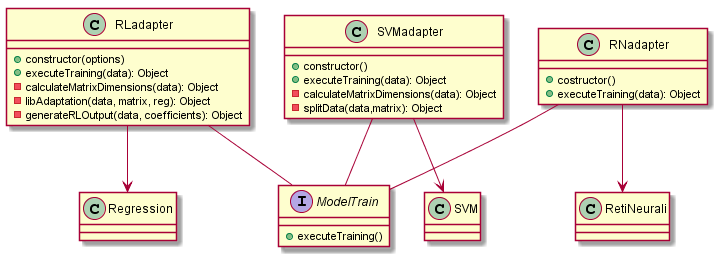
\includegraphics[width=14cm]{img/classDiagramRN.png}
              \label{fig:scice_documenti}
              \caption{Esempio aggiunta class adapter per Reti neurali}
            \end{figure}
  \item Ultimo passaggio, opzionale, è quello di creare dei metodi privati di ausilio per il metodo executeTraining(data) in modo anche da facilitare la leggibilità del codice creato.
            \begin{figure}[H]
              \centering
              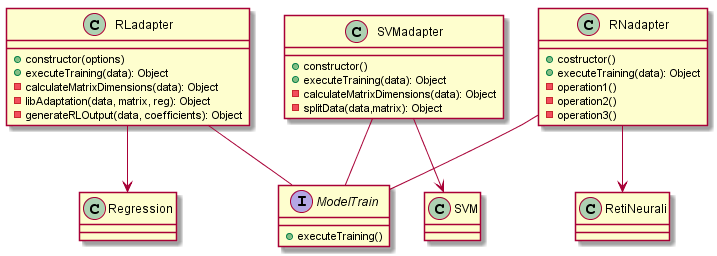
\includegraphics[width=14cm]{img/classDiagramRNoperation.png}
              \label{fig:scice_documenti}
              \caption{Esempio aggiunta metodi privati nella classe RNadapter}
            \end{figure}
\end{enumerate}


\end{document}
